%!TEX root = ../Main.tex
\section{Appendix}
\appendix
\section*{Figures}
%
\begin{figure}[!htbp]\caption{\ac{SPX} and VIX}\label{fig:SPandVIX}
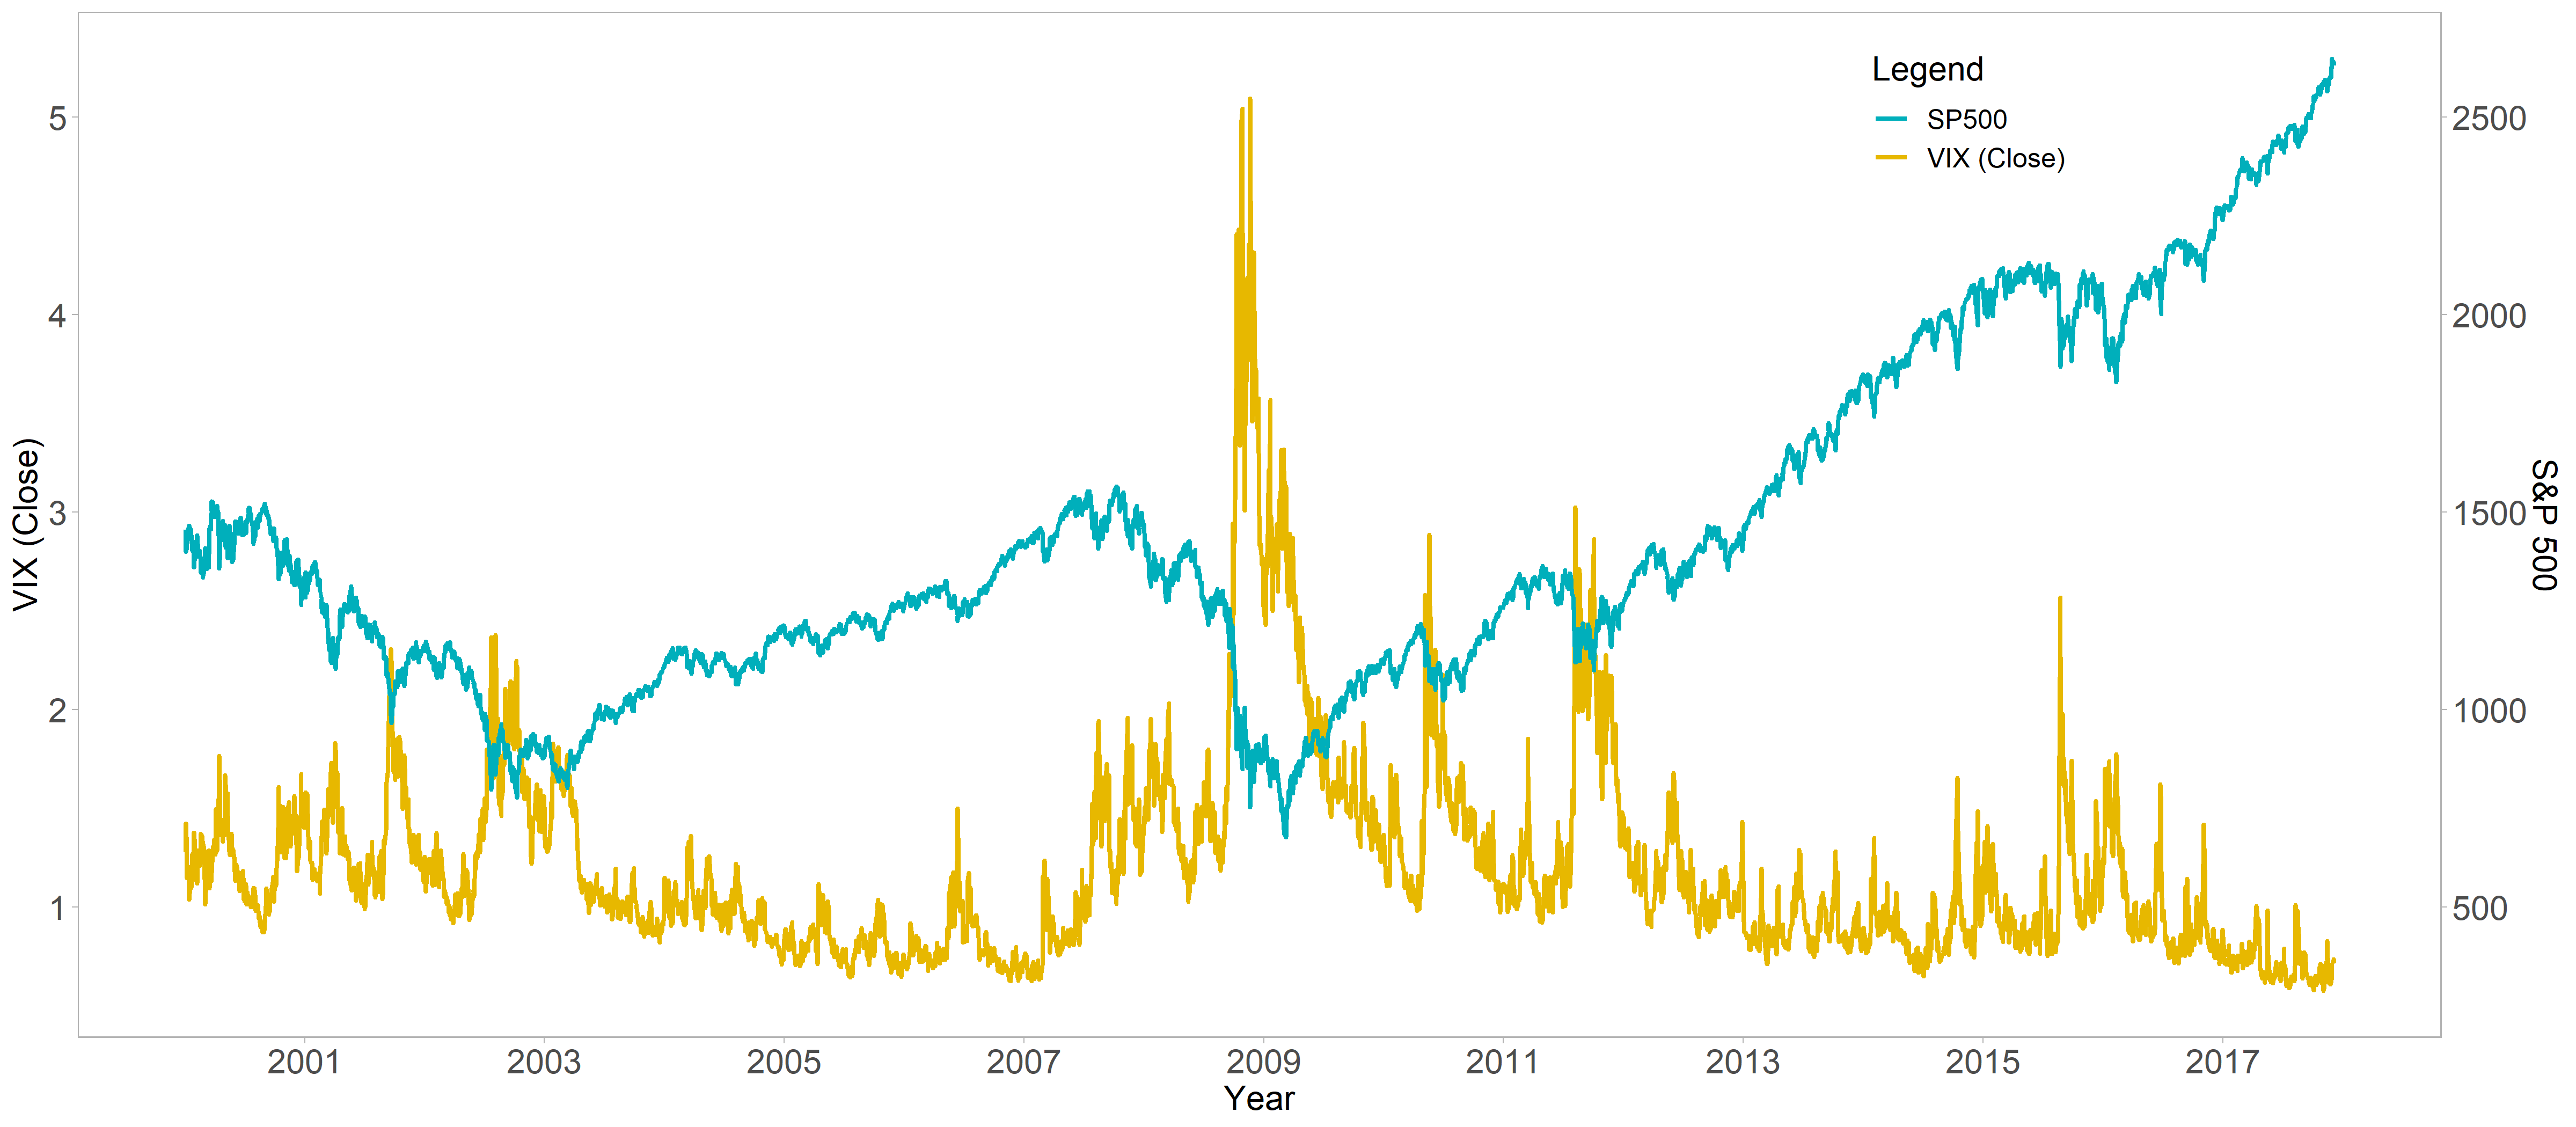
\includegraphics[width=16cm, height=8cm]{pictures/SPandViX.png}
\end{figure}
%
\begin{figure}[!htbp]\caption{\ac{SPX} and RV and VIX}\label{fig:SPandVIXandVol}
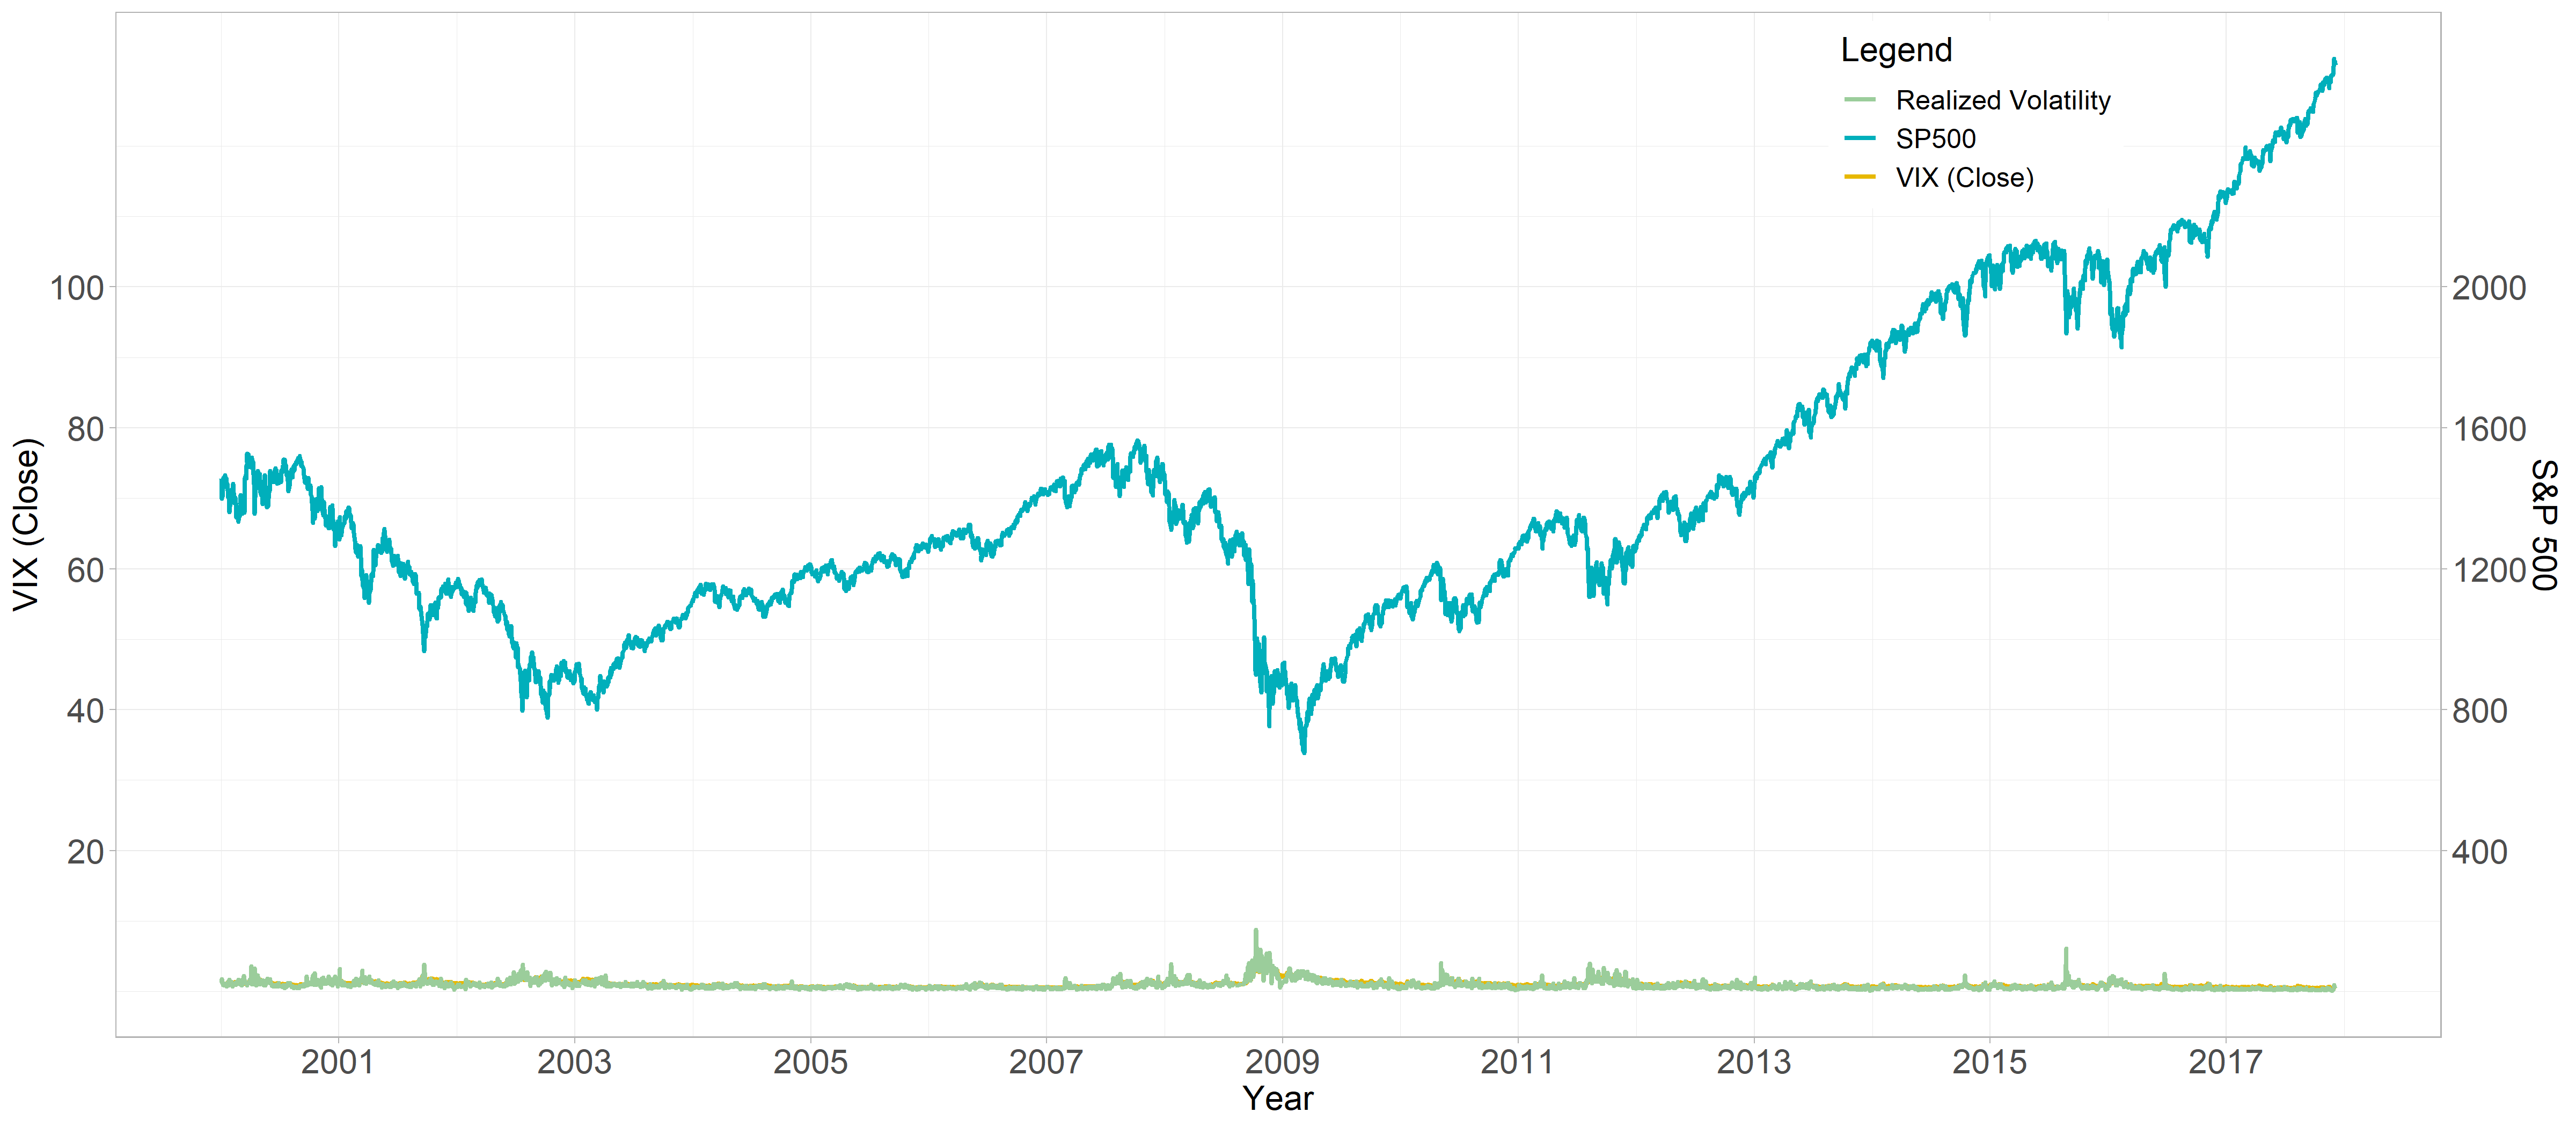
\includegraphics[width=16cm, height=8cm]{pictures/SPandVolandViX.png}
\end{figure}

\newpage
\section*{Data Summary Statistics}
% Table created by stargazer v.5.2.2 by Marek Hlavac, Harvard University. E-mail: hlavac at fas.harvard.edu
% Date and time: Fr, Jan 11, 2019 - 17:33:58
\begin{table}[!htbp] \centering 
  \caption{Summary statistics: Variables} 
  \label{tab:summary1} 
\begin{tabular}{@{\extracolsep{5pt}}lccccccc} 
\\[-1.8ex]\hline 
\hline \\[-1.8ex] 
Statistic & \multicolumn{1}{c}{N} & \multicolumn{1}{c}{Min} & \multicolumn{1}{c}{Max} & \multicolumn{1}{c}{Mean} & \multicolumn{1}{c}{St. Dev.} & \multicolumn{1}{c}{Skewness} & \multicolumn{1}{c}{Kurtosis} \\
\hline \\[-1.8ex] 
\multicolumn{8}{c}{All time periods} \\
\hline \\[-1.8ex] 
RV & 4,434 & 0.110 & 8.802 & 0.874 & 0.615 & 3.127 & 17.751 \\ 
VIX & 4,434 & 0.576 & 5.094 & 1.196 & 0.525 & 2.552 & 9.787 \\ 
Weekly RV & 4,434 & 0.183 & 5.586 & 0.874 & 0.556 & 2.757 & 12.451 \\ 
Monthly RV & 4,434 & 0.223 & 4.375 & 0.876 & 0.512 & 2.534 & 10.051\\ 
Weekly VIX & 4,434 & 0.596 & 4.593 & 1.197 & 0.519 & 2.510 & 9.235 \\ 
Monthly VIX & 4,434 & 0.618 & 4.126 & 1.198 & 0.504 & 2.491 & 8.853 \\ 
\hline \\[-1.8ex] 
\multicolumn{8}{c}{During crisis} \\
\hline \\[-1.8ex] 
RV & 1,252 & 0.213 & 8.802 & 1.171 & 0.834 & 2.713 & 11.399\\ 
VIX  & 1,259 & 0.847 & 5.094 & 1.623 & 0.695  & 1.941 &  4.232\\ 
Weekly RV & 1,259 & 0.257 & 5.586 & 1.169 & 0.753 & 2.409 & 7.417\\ 
Monthly RV & 1,259 & 0.423 & 4.375 & 1.172 & 0.689 & 2.178 & 5.448\\ 
Weekly VIX & 1,259 & 0.885 & 4.593 & 1.623 & 0.684  &  1.885 & 3.753\\ 
Monthly VIX & 1,259 & 0.946 & 4.126 & 1.625 & 0.662 & 1.837 & 3.311\\ 
\hline \\[-1.8ex] 
\multicolumn{8}{c}{Outside of crisis} \\
\hline \\[-1.8ex] 
RV & 3,229 & 0.110 & 6.109 & 0.762 & 0.454 & 2.252 & 10.798\\ 
VIX & 3,251 & 0.576 & 2.566 & 1.034 & 0.307 & 1.206 & 1.365 \\ 
Weekly RV & 3,246 & 0.183 & 3.165 & 0.765 & 0.400 & 1.564 &  3.441\\ 
Monthly RV & 3,229 & 0.223 & 2.367 & 0.764 & 0.363 & 1.308 & 1.687  \\ 
Weekly VIX & 3,246 & 0.596 & 2.188 & 1.034 & 0.300  & 1.157 &  1.047 \\ 
Monthly VIX & 3,229 & 0.618 & 2.014 & 1.033 & 0.285 &  1.1 & 0.78\\ 
\hline \\[-1.8ex] 
\end{tabular} 
\end{table} 

\newgeometry{left=1cm, right=1cm, top=2cm, bottom=1cm}

% Table created by stargazer v.5.2.2 by Marek Hlavac, Harvard University. E-mail: hlavac at fas.harvard.edu
% Date and time: Fr, Jan 11, 2019 - 18:36:21
\begin{table}[!htbp] \centering 
  \caption{Summary statistics: Logarithm variables} 
  \label{tab:summary2} 
\begin{tabular}{@{\extracolsep{5pt}}lccccccc} 
\\[-1.8ex]\hline 
\hline \\[-1.8ex] 
Statistic & \multicolumn{1}{c}{N} & \multicolumn{1}{c}{Min} & \multicolumn{1}{c}{Max} & \multicolumn{1}{c}{Mean} & \multicolumn{1}{c}{St. Dev.} & \multicolumn{1}{c}{Skewness} & \multicolumn{1}{c}{Kurtosis} \\ 
\hline \\[-1.8ex] 
\multicolumn{8}{c}{All time periods} \\
\hline \\[-1.8ex] 
RV & 1,236 & $-$9.664 & 0.777 & $-$1.469 & 1.262 & -1.369 & 3.185 \\ 
VIX & 2,528 & $-$8.005 & 0.487 & $-$1.562 & 1.190 & -1.294 & 2.586\\ 
Weekly RV & 4,434 & 0.183 & 5.586 & 0.874 & 0.556  &  2.757 & 12.451\\ 
Monthly RV & 4,434 & $-$1.501 & 1.476 & $-$0.259 & 0.483 &  0.487 & 0.357  \\ 
Weekly VIX & 4,434 & $-$0.518 & 1.525 & 0.111 & 0.350 & 0.933 &  1.117  \\ 
Monthly VIX & 4,434 & $-$0.481 & 1.417 & 0.115 & 0.340 &  0.963 &   1.227\\ 
\hline \\[-1.8ex] 
\multicolumn{8}{c}{During crisis} \\
\hline \\[-1.8ex] 
RV & 1,252 & 0.213 & 8.802 & 1.171 & 0.834 & 2.713 & 11.399\\ 
VIX & 1,259 & 0.847 & 5.094 & 1.623 & 0.695 & 1.941 & 4.232 \\ 
Weekly RV & 1,259 & 0.257 & 5.586 & 1.169 & 0.753 &  2.409 & 7.417 \\ 
Monthly RV & 1,259 & 0.423 & 4.375 & 1.172 & 0.689 & 2.178 & 5.448\\ 
Weekly VIX & 1,259 & 0.885 & 4.593 & 1.623 & 0.684 &  1.885 &  3.753\\ 
Monthly VIX & 1,259 & 0.946 & 4.126 & 1.625 & 0.662 &  1.837 &  3.311\\ 
\hline \\[-1.8ex] 
\multicolumn{8}{c}{Outside of crisis} \\                           
\hline \\[-1.8ex] 
RV & 3,229 & 0.110 & 6.109 & 0.762 & 0.454 & 2.252  & 10.798\\ 
VIX & 3,251 & 0.576 & 2.566 & 1.034 & 0.307 & 1.206 & 1.365\\ 
Weekly RV & 3,246 & 0.183 & 3.165 & 0.765 & 0.400  &  1.564  & 3.441 \\ 
Monthly RV & 3,229 & 0.223 & 2.367 & 0.764 & 0.363  & 1.308 & 1.687\\ 
Weekly VIX & 3,246 & 0.596 & 2.188 & 1.034 & 0.300  & 1.157 & 1.047\\ 
Monthly VIX & 3,229 & 0.618 & 2.014 & 1.033 & 0.285 & 1.100 & 0.780 \\ 
\hline \\[-1.8ex] 
\end{tabular} 
\end{table} 

% Table created by stargazer v.5.2.2 by Marek Hlavac, Harvard University. E-mail: hlavac at fas.harvard.edu
% Date and time: Sa, Jan 12, 2019 - 09:20:14
\begin{table}[!htbp] \centering 
  \caption{Correlation table} 
  \label{tab:correlation} 
\begin{tabular}{@{\extracolsep{5pt}} ccccccccc} 
\\[-1.8ex]\hline 
\hline \\[-1.8ex] 
 & RV & VIX & Daily RV & Weekly RV & Monthly RV & D. VIX & W.VIX & M. VIX \\ 
\hline \\[-1.8ex] 
RV & $1$ & $0.837$ & $0.806$ & $0.823$ & $0.769$ & $0.819$ & $0.781$ & $0.698$ \\ 
VIX & $0.837$ & $1$ & $0.822$ & $0.883$ & $0.903$ & $0.981$ & $0.969$ & $0.926$ \\ 
Daily RV & $0.806$ & $0.822$ & $1$ & $0.890$ & $0.794$ & $0.837$ & $0.803$ & $0.710$ \\ 
Weekly RV & $0.823$ & $0.883$ & $0.890$ & $1$ & $0.903$ & $0.896$ & $0.906$ & $0.809$ \\ 
Monthly RV & $0.769$ & $0.903$ & $0.794$ & $0.903$ & $1$ & $0.910$ & $0.932$ & $0.931$ \\ 
Daily VIX & $0.819$ & $0.981$ & $0.837$ & $0.896$ & $0.910$ & $1$ & $0.982$ & $0.935$ \\ 
Weekly VIX & $0.781$ & $0.969$ & $0.803$ & $0.906$ & $0.932$ & $0.982$ & $1$ & $0.961$ \\ 
Monthly VIX & $0.698$ & $0.926$ & $0.710$ & $0.809$ & $0.931$ & $0.935$ & $0.961$ & $1$ \\ 
\hline \\[-1.8ex] 
\end{tabular} 
\end{table} 

\restoregeometry
%\newgeometry{left=2cm, right=2cm, top=2cm, bottom=1cm}
\section*{Regression Results with Robustness Checks}

% Table created by stargazer v.5.2.2 by Marek Hlavac, Harvard University. E-mail: hlavac at fas.harvard.edu
% Date and time: Sa, Jan 19, 2019 - 20:40:21
\begin{table}[!htbp] \centering 
  \caption{Level regression (whole sample)} 
  \label{newey1} 
\begin{tabular}{@{\extracolsep{5pt}}lccc} 
\\[-1.8ex]\hline 
\hline \\[-1.8ex] 
 & \multicolumn{3}{c}{\textit{Dependent variable:}} \\ 
\cline{2-4} 
\\[-1.8ex] & \multicolumn{3}{c}{Realized Volatility} \\ 
 & Reg1a & Reg2a & Reg3a \\ 
\\[-1.8ex] & (1) & (2) & (3)\\ 
\hline \\[-1.8ex] 
 Intercept & 0.045$^{***}$ & $-$0.324$^{***}$ & $-$0.169$^{***}$ \\ 
  & (0.015) & (0.059) & (0.034) \\ 
  & & & \\ 
 $RV^{(d)}_{t}$ & 0.362$^{***}$ &  & 0.256$^{***}$ \\ 
  & (0.038) &  & (0.040) \\ 
  & & & \\ 
 $RV^{(w)}_{t}$ & 0.391$^{***}$ &  & 0.286$^{***}$ \\ 
  & (0.056) &  & (0.064) \\ 
  & & & \\ 
 $RV^{(m)}_{t}$ & 0.188$^{***}$ &  & $-$0.106$^{**}$ \\ 
  & (0.036) &  & (0.050) \\ 
  & & & \\ 
 $crisis$ & 0.025$^{*}$ & $-$0.214$^{***}$ & $-$0.112$^{***}$ \\ 
  & (0.013) & (0.035) & (0.021) \\ 
  & & & \\ 
 $VIX_{t}$ &  & 1.052$^{***}$ & 0.579$^{***}$ \\ 
  &  & (0.059) & (0.064) \\ 
  & & & \\ 
\hline \\[-1.8ex] 
AIC & 2817.4 & 3104.2 & 2446 \\ 
Observations & 4,434 & 4,434 & 4,434 \\ 
R$^{2}$ & 0.708 & 0.689 & 0.732 \\ 
Adjusted R$^{2}$ & 0.708 & 0.688 & 0.732 \\ 
Residual Std. Error & 0.332 (df = 4429) & 0.343 (df = 4431) & 0.319 (df = 4428) \\ 
\hline 
\hline \\[-1.8ex] 
\textit{Note:}  & \multicolumn{3}{r}{$^{*}$p$<$0.1; $^{**}$p$<$0.05; $^{***}$p$<$0.01} \\ 
\end{tabular} 
\end{table} 


% Table created by stargazer v.5.2.2 by Marek Hlavac, Harvard University. E-mail: hlavac at fas.harvard.edu
% Date and time: Di, Jan 15, 2019 - 16:19:13
\begin{table}[!htbp] \centering 
\begin{threeparttable}
  \caption{Level regression} 
  \label{tab:overlap1} 
\begin{tabular}{@{\extracolsep{5pt}}lccc} 
\\[-1.8ex]\hline 
\hline \\[-1.8ex] 
 & \multicolumn{3}{c}{\textit{Dependent variable:}} \\ 
\cline{2-4} 
\\[-1.8ex] & \multicolumn{3}{c}{Realized Volatility} \\ 
 & Reg1a & Reg2a & Reg3a \\ 
\\[-1.8ex] & (1) & (2) & (3)\\ 
\hline \\[-1.8ex] 
 Intercept & 0.046 & $-$0.342$^{***}$ & $-$0.134$^{**}$ \\ 
  & (0.031) & (0.091) & (0.052) \\ 
  & & & \\ 
 $RV^{d}_{t}$ & 0.408$^{***}$ &  & 0.330$^{***}$ \\ 
  & (0.109) &  & (0.116) \\ 
  & & & \\ 
 $RV^{w}_{t}$ & 0.501$^{***}$ &  & 0.394$^{***}$ \\ 
  & (0.126) &  & (0.128) \\ 
  & & & \\ 
 $RV^{m}_{t}$ & 0.072 &  & $-$0.132 \\ 
  & (0.079) &  & (0.083) \\ 
  & & & \\ 
 $crisis$ & $-$0.022 & $-$0.257$^{***}$ & $-$0.131$^{***}$ \\ 
  & (0.029) & (0.058) & (0.035) \\ 
  & & & \\ 
 $VIX_{t}$ &  & 1.092$^{***}$ & 0.460$^{***}$ \\ 
  &  & (0.094) & (0.089) \\ 
  & & & \\ 
\hline \\[-1.8ex] 
AIC & 192.5 & 281.8 & 166 \\ 
Observations & 456 & 456 & 456 \\ 
R$^{2}$ & 0.757 & 0.701 & 0.771 \\ 
Adjusted R$^{2}$ & 0.754 & 0.700 & 0.769 \\ 
Residual Std. Error & 0.297 (df = 451) & 0.328 (df = 453) & 0.288 (df = 450) \\ 
\hline 
\hline \\[-1.8ex] 
\textit{Note:}  & \multicolumn{3}{r}{$^{*}$p$<$0.1; $^{**}$p$<$0.05; $^{***}$p$<$0.01} \\ 
\end{tabular} 
 \begin{tablenotes}
      \small
      \item The numbers in the brackets are the standard errors of the parameters computed with Newey-West covariance correction, which are robust to autocorrelated and heteroscedastic error terms, see \textcite{newey1987}.
    \end{tablenotes}
  \end{threeparttable}
\end{table} 


% Table created by stargazer v.5.2.2 by Marek Hlavac, Harvard University. E-mail: hlavac at fas.harvard.edu
% Date and time: So, Jan 13, 2019 - 10:25:28
\begin{table}[!htbp] \centering 
  \caption{logarithmic regression} 
  \label{} 
\begin{tabular}{@{\extracolsep{5pt}}lccc} 
\\[-1.8ex]\hline 
\hline \\[-1.8ex] 
 & \multicolumn{3}{c}{\textit{Dependent variable:}} \\ 
\cline{2-4} 
\\[-1.8ex] & \multicolumn{3}{c}{Realized Volatility} \\ 
 & Reg1b & Reg2b & Reg3b \\ 
\\[-1.8ex] & (1) & (2) & (3)\\ 
\hline \\[-1.8ex] 
 c & $-$0.001 & $-$0.364$^{***}$ & $-$0.049$^{*}$ \\ 
  & (0.018) & (0.026) & (0.028) \\ 
  & & & \\ 
 $ ln(RV^{d}_{t})$ & 0.346$^{***}$ &  & 0.352$^{***}$ \\ 
  & (0.064) &  & (0.064) \\ 
  & & & \\ 
 $ln(RV^{w}_{t})$ & 0.408$^{***}$ &  & 0.432$^{***}$ \\ 
  & (0.078) &  & (0.080) \\ 
  & & & \\ 
 $ ln(RV^{m}_{t})$ & 0.171$^{***}$ &  & 0.003 \\ 
  & (0.054) &  & (0.088) \\ 
  & & & \\ 
 $crisis$ & $-$0.017 & $-$0.169$^{***}$ & $-$0.063$^{*}$ \\ 
  & (0.027) & (0.062) & (0.034) \\ 
  & & & \\ 
 $ln(VIX_{t})$ &  & 1.229$^{***}$ & 0.236$^{**}$ \\ 
  &  & (0.074) & (0.104) \\ 
  & & & \\ 
\hline \\[-1.8ex] 
AIC & 126.4 & 415.1 & 123.9 \\ 
Observations & 456 & 455 & 455 \\ 
R$^{2}$ & 0.748 & 0.522 & 0.751 \\ 
Adjusted R$^{2}$ & 0.746 & 0.519 & 0.748 \\ 
Residual Std. Error & 0.276 (df = 451) & 0.380 (df = 452) & 0.275 (df = 449) \\ 
\hline 
\hline \\[-1.8ex] 
\textit{Note:}  & \multicolumn{3}{r}{$^{*}$p$<$0.1; $^{**}$p$<$0.05; $^{***}$p$<$0.01} \\ 
\end{tabular} 
\end{table} 


\section*{F-test Results with Robustness Checks}
% latex table generated in R 3.5.1 by xtable 1.8-3 package
% Wed Jan 16 11:15:10 2019
\begin{table}[ht]
\centering
\caption{F-test Reg3a} 
\begin{tabular}{lrrrrrr}
  \hline
 & Res.Df & RSS & Df & Sum of Sq & F & Pr($>$F) \\ 
  \hline
1 & 4432 & 524.31 &  &  &  &  \\ 
  2 & 4428 & 449.29 & 4 & 75.03 & 184.86 & 0.0000 \\ 
   \hline
\end{tabular}
\end{table}

% latex table generated in R 3.5.1 by xtable 1.8-3 package
% Sun Jan 20 01:19:32 2019
\begin{table}[htbp!]
\centering
\caption{F-test Reg3b} 
\begin{tabular}{lrrrrrr}
  \hline
 & Res.Df & RSS & Df & Sum of Sq & F & Pr($>$F) \\ 
  \hline
1 & 4432 & 529.46 &  &  &  &  \\ 
  2 & 4428 & 367.22 & 4 & 162.24 & 489.09 & 0.0000 \\ 
   \hline
\end{tabular}
\end{table}

% latex table generated in R 3.5.1 by xtable 1.8-3 package
% Wed Jan 16 16:54:16 2019
\begin{table}[htbp!]
\centering
\caption{F-test Reg3a non-overlapping sample} 
\begin{tabular}{lrrrrrr}
  \hline
 & Res.Df & RSS & Df & Sum of Sq & F & Pr($>$F) \\ 
  \hline
1 & 4432 & 524.31 &  &  &  &  \\ 
  2 & 4428 & 449.29 & 4 & 75.03 & 184.86 & 0.0000 \\ 
   \hline
\end{tabular}
\end{table}

% latex table generated in R 3.5.1 by xtable 1.8-3 package
% Wed Jan 16 11:15:11 2019
\begin{table}[ht]
\centering
\caption{F-test Reg3b non-overlapping sample} 
\begin{tabular}{lrrrrrr}
  \hline
 & Res.Df & RSS & Df & Sum of Sq & F & Pr($>$F) \\ 
  \hline
1 & 4432 & 529.46 &  &  &  &  \\ 
  2 & 4428 & 367.22 & 4 & 162.24 & 489.09 & 0.0000 \\ 
   \hline
\end{tabular}
\end{table}

%\restoregeometry
%\clearpage



